%%%%%%%%%%%%%%%%%%%%%%%%%%%%%%%%%%%%%%%%%%%%%%%%%%%%%%%%%%%%%%%%%%%
% Method
% Team:
% Union
% Members: 
% Bernie Huang, Jim Lan, Hoang Tan, Kenny Hsu, Rahul Aditya, Tan Phat, Wei
% Relative files:
% Method_Union.tex
% Note:    
% Do not compile this file compile Main.tex to get the pdf file instead.
%%%%%%%%%%%%%%%%%%%%%%%%%%%%%%%%%%%%%%%%%%%%%%%%%%%%%%%%%%%%%%%%%%%
\subsection{Method} %Please change "Method" to your goal. 
\textit{\footnotesize Author:Bernie Huan, Jim Lan, Hoang Tan, Kenny Hsu, Rahul Aditya, Tan Phat, Wei.}\\

As mentioned in the background, our team used natural language processing in order to generate metadata. 
The scope of metadata processing is about producing at least three types of metadata including author name, title and abstract.
This is the least we want to do within the time frame of this course.
Once accomplishing the 3 types of metadata, we will extend the scope of our project, intimidate the scheme to produce other remaining metadata such as doix number, journal name, volume number and so on.
If time is still on our side, we will even extend the scope of our project further and join other teams to produce a search engine.
Following discussion are our plan to complete extracting the 4 first types of metadata from PDF files.

\subsubsection{Title extraction}

We chose python to be the program to catch the title and other metadata.
First step, we import some necessary packages and functions as following:

\begin{enumerate}
	
	\item re: Regular expression package is a useful package which could be applied to the string comparison.
	\item os: This function can connect the python to operating system, so that we can call the path of the files and folders.
	\item nltk: A natural language toolkit.	We use the corpus plaintext function to build the txt file in a folder as corpus.
	\item string:The string package includes a lot of classes such as lowercase, uppercase,punctuation,digits or whitespace...etc.
	
\end{enumerate}  

To begin, all PDF files are converted into txt file with which we want to deal with.
The path is set and the files are stored in a specific folder.
Then, regular expression in python can help capturing the first sentence in the txt files, which have been converted and stored in specific folder in previous step.
The process of extracting title from the text is mainly regulated by Union\_extract\_title.py.
The coding scheme has following steps:Importation of necessary components, setting the path, creating the directory we will write the .txt files to after stripping text, using basic command to extract titles.
The results are tested and listed.
We successfully produce the title of the article in the txt file. 

\subsubsection{Author extraction}

In this part, we use the existing python packages to achieve our goal.
The key point in this part is natural language processing, 
which we have introduced in the basic section.
Also we combine the key word comparison technique to finish this task.
The following step is below:

\begin{enumerate}
	
	\item Section Separation: As we separate the abstract part from the full text, we extract the text above the 
	abstract section and rename as top section. 
	This section contains title, author and email ,etc.
	\item Tokenization: After accessing the top section, we separate the text into each single word. 
	These single words composed with a string list. 
	\item Part Of Speech Tag: We use the existing corpus to tag the part of speech to the words. 
	This step is necessary since that the chunker needs the every word's part-of-speech and then chunck.
	\item Chunker: In this part, we mainly chunk the noun because a noun often represents some meaningful features 
	such as location or author.
	\item Label: We check every phrase with the corpus which contain specific words like people name. 
	Then we label the words and store within the new list. 
	Eventually, we write the information within the xml file. 
	
\end{enumerate}

The above steps is also available to extracting the location and organization,etc 
when needed. 
The file mainly functioning for this task is Extract\_Authors.py.
The coding scheme for this task is quite similar to title extraction.
The main different is a corpus is introduced.
This scheme also include a natural language toolkit in order to extract people's name. 
As we test the result, our program has been able to extract authors' name.

\subsubsection{Abstract extraction}

Developing from previous theory mentioned in the background section, 
we use the python to catch the abstract.
The following step is below.
%\begin{center}
%	\includegraphics[width=\columnwidth]{Union_Background_Chart_2
%\end{center}
The pdf is converted into txt file.
Thus, it will create the txt file.
The work is done by hand coding.
For detailed coding scheme, we have presented it in the appendix at the end of this report.

After being able to read the txt file on every line, 
the python will detect the content of the abstract.
In order to do so, we strip the text between "abstract" label and "introduction" label.	


Abstract-database:including the condition

\begin{enumerate}
	
	\item Capital         "ABSTRACT".
	\item Lower case      "abstract".
	\item In the sentence "Abstract—Word sense ...".
	\item And so on...
	
\end{enumerate}

In the process building "abstract database", we are aware of different papers may have different form of structures 
and writing style, we search through numbers of articles from different journals.
Number of article found is 100, from 20 different journals including The Lancet, Progress in Energy and Combustion Science, Chemical Analysis and so.
Search results for sections such as Theoretical, Methods, Results, Discussion, Conclusion, Acknowledgments are also obtained.
Table below are the results of the search.

%\begin{center}
%\includegraphics[width=\columnwidth]{Table for method Union}.\\
%\includegraphics[width=\columnwidth]{Table 2 for method Union}.\\
%\caption{Result of finding all forms of "abstract", "introduction" written by different authors}
%\end{center}

Then our program will read the txt file on every line.
If the python detects the abstract-database-stop's words ,
it will stop to catch the sentences.
abstract-database-stop:including the following conditions

\begin{enumerate}
	
	\item The blank line.
	\item Specific words in the beginning "Keywords".
	\item And so on.
	
\end{enumerate}

The intended output are sentences extracted to the txt file.
To further validate if the program can run precisely, members randomly search for articles (10 articles) to test the programs.
The program was run successfully and all abstracts was extracted from the text.

\subsubsection{References URL extraction}

References URL extraction is very easy and straightforward.
Just use a powerful package called PDfx to complete this task.
Find the package online and use it.
The procedures are below:

\begin{enumerate}
	
	\item First of all, a PDFx package is imported to python.
	\item Second, The function in PDFx package is utilized to get the metadata and the URL of references by inputting a URL of a PDF or PDF's file name.
	\item Finally, output and list the results in txt file and choose the specific directory to store it.
	
\end{enumerate}

This method can also detects URL,arxiv and doi references.  
Plus,by using this method, we also can easily extract the title, page number and creation date. 
However,only the page number is always right in every case. 
The others are not totally correct. 
Basically, over 50 percent is not correct.
Thus, among these metadata,this method is more suitable for page number. 

\subsubsection{Search sentences}

The search sentence part is related to the search engine.
After extracting the necessary information, we have to find a way to search these data.
The procefure is following:
\begin{itemize}
	
	%\begin{center}
	%	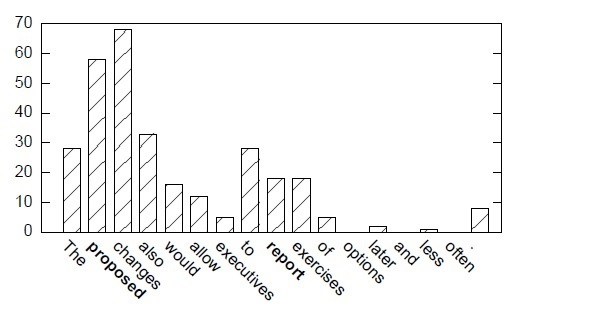
\includegraphics[width=0.8\columnwidth]{Union_Background_Chart_2}
	%\end{center}
	\item First, The PDF is converted to the txt file.(Make the program to read the file name much easier)
	\item Second, read the txt files by lines.
	\item Third, the array is created to divide the section of the articles.
	\item Fourth, The array is expanded to divide the section clearly.
	\item Fifth, Users search the sentences, the program search all the sections by this sentence.
	\item Sixth, show the results.
	
\end{itemize}
\subsection{API}
We also attempt to produce an semi-automatic interface that help users to inquire certain information from our database. 
Currently it allows user to search for abstracts, introduction, method, result, discussion, and reference. We will continue develop the interface in the remaining week. 
The objectives are either covering more functions or make the results pages has more professional appearance. However, that
said when we still have enough time.

\newpage % Ends the current page and causes all figures and tables to be printed